\section{Histoire du DICOM}

	\frame
	{
		\frametitle{Pr�histoire}
		
		\begin{itemize}
			\item Arriv�e du num�rique en m�decine.
			\item Stockage, transmission, affichage des images : constructeur d�pendant.
			\item Solutions propri�taires (par opposition � solutions ouvertes) :
			\begin{itemize}
				\item argument commercial : "Mon protocole est meilleur que les autres", "Nos produits ont une excellente interaction entre eux", "Nous g�rons tout de A � Z" ;
				\item interaction impossible entre marques diff�rentes.
			\end{itemize} 
			\item Cons�quences :
			\begin{itemize}
				\item pi�ge commercial : obligation d'acqu�rir les stations d'acquisition et de traitement ad�quates, et changer de marque peut rendre les anciens examens illisibles ;
				\item pi�ge m�dical : difficile de communiquer entre coll�gues.
			\end{itemize}
		\end{itemize}
	}
					
	\frame
	{
		\frametitle{D�buts du DICOM}
		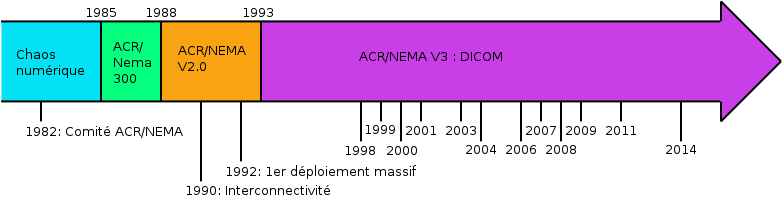
\includegraphics[width=\linewidth]{./figures/chrono-dicom.png}

		\begin{itemize}
			\item 1\up{�re} version ACR/NEMA 300 en 1985 : peu accept� car vague et contenant des incoh�rences.
			\item 2\up{�me} version en 1988 : transmission des images par le connecteur mat�riel EIA-485, adopt� par quelques constructeurs.
			\item 3\up{�me} version en 1993 : ind�pendance du connecteur, donc support TCP.
		\end{itemize}
	}
	
	\frame
	{
		\frametitle{Support / Sponsoring}
		\begin{itemize}
			\item ACR : American College of Radiology
			\item NEMA : National Electrical Manufacturers Association
			\item JIRA : Japan Investor Relations Association
			\item CEN : Comit� Europ�en de Normalisation
			\item IEEE, HL7, ANSI,?
		\end{itemize}
	}

	\frame
	{
		\frametitle{DICOM aujourd'hui}
		\begin{itemize}
			\item Standard accept� mondialement.
			\item Actuellement en version $2011$ : on parle des versions par leur ann�e (officiellement, toujours en version 3 � PS3)
			\item Diversit� des �quipements support�s : RX, CT, IRM, US, PET, SPECT, Angio, ECG,?
			\item Adopt� par de nombreux constructeurs : GE, Siemens, Philips, Toshiba,?
		\end{itemize}
	}
